\documentclass[letterpaper]{article}
\usepackage{graphicx}
\usepackage{outline}
\begin{document}

\title{A protocol for implementing read-only databases in dynamic distributed environments}
\author{Adam Drescher \and Magdalena Cassel}
\date{}

\maketitle

\begin{abstract}
The abstract abstract.
\end{abstract}

\section{Introduction}

Dynamic distributed systems are often governed by immutable or slowly changing configuration information contributed by each node in the system.
A common problem is listing all of the participants

For example, systems that use discovery and advertisement are governed by service specifications and descriptions contributed by service consumers and providers.
%  A recurring problem in dynamic distributed systems is the collection and processing of configuration information.

Both centralized and distributed algorithms have been proposed to collect and process configuration information.
Centralized algorithms elect a leader which then facilitates the collection of configuration information and query processing.
The leader might perform the processing itself or delegate processing to a subordinate.
Distributed algorithms for configuration information collection and processing often use one of two techniques depending on the size of the records.
If the records are bigger than the size of a message in the network, i.e., a UDP packet, then nodes discover other nodes using broadcast messages and then use point-to-point connections to collect and process the configuration information.
If the records are smaller than the size of a message in the network, then the nodes exchange data using a multicast network, e.g., the Multicast Domain Name System.

An unexplored area of the design space is techniques that support 

The problem of processing the configuration information can be cast using database techniques.
Continuing the example, a service specification is a record in a table of service specifications and the process of discovery involves projecting the specification record on to the table of service descriptions.



A recurring problem in dynamic distributed environments Read-only datab

Dynamic distributed systems often require a protocol that allows a node to share public immutable data with all of the other nodes in the system.
A typical example is discovery where service specifications are compared against service descriptions to match service providers with service consumers.
Service descriptions and specifications are immutable even though they might exist at different times in the system since the set of nodes and therefore service providers and consumers may change with time.
The immutability and public nature of the data implies that it can be freely replicated and therefore learned by gossiping.






Often, the number of times the data is read is proportional to the number of nodes.





There's a number of ways to do this.
1.  Centralized approach where a leader becomes a data broker
2.  Discover other nodes and then poll them.

The main problem with the first approach is that its centralized.
A problem with the second approach is that its inefficient (if you are n then you will be contacted n - 1 times).

By dynamic, we mean that components come in and out.

We assume a moderately sized ad hoc wireless network.

We would like to take advantage of gossip.
We would like to be fully distributed.

Thus we developed a dissemination protocol for remote data exchange in wireless networks.

Moving data across a network can take a variety of forms. 
These forms correspond to different user needs and consequently different protocols. 
Multicast File Transfer Protocol (MFTP) addresses the need to move immutable data between many different nodes in a fully distributed network. 
%% This is useful for 1) device discovery 2) File transfer in the absence of many technologies (including internet). the only thing that is necessary is computers with routing and broadcast/multicast enabled 3) maximizing the reach of a gossip style network

\section{Model\label{model}}

\paragraph {Files.}
The main concept in MFTP is that of a \emph{file}.
A file is a sequence of bytes with a length and a user-defined type.
Files are broken down into pieces of equal size called \emph{fragments}.
Each file is uniquely identified by a \emph{file ID} that contains the file's type, length, and a hash of the file's content.
% TODO:  We need to move this.
% Given two files $f_1$ and $f_2$, one can define a matching predicate $\mu$.

\paragraph{Messages.}
File transfer takes place via \emph{messages}.
There are three types of messages in the protocol.
The first message type is a \emph{request}.
A request contains a file ID and a set of fragment indices.
We implemented requests as the file ID and a set of contiguous regions.  
However, one can envision the request to contain anything that defines a set.
The second message type is a \emph{fragment}, which consists of a file ID, a fragment index, and the data comprising that fragment of the file.
Last is a \emph{match}, which consists of a file ID and a set of matching file IDs.

\paragraph {Tasks.}
MFTP is a peer-to-peer protocol because each participant can act as both a client and a server.
A peer can send out any fragments for which it gets a request.
Fragments are periodically broadcast, even in the absence of requests, to indicate what files exist in the network.
A peer can use requests to poll for fragments of a file which can span from individual fragments to the whole file.
A peer which has successfully downloaded any number of fragments of a file can then serve those fragments.

Matching is a two-step process.
The first step applies a matching function $\iota$ to two file IDs to determine whether a match is possible between the two files.  
The second step applies a matching function $\mu$ to the two files to determine whether there is a match.
If $\mu$($f_1$,$f_2$) is true, $\iota$($fid_1$,$fid_2$) must be true.
However, if $\iota$($fid_1$,$fid_2$) is true, $\mu$($f_1$,$f_2$) does \emph{not} have to be true. 

%%TODO: Talk about validation

\section{Implementation}

%%TODO: Talk about validation - possible coinage 'incremental digest'

\paragraph{MFTP Automaton.}
Our implementation of MFTP uses the ioa framework.
I/O Automata model stateful distributed system components that can interact and be composed with each other.
They change state through transitions classified as input, output or internal actions.
Input and output actions in different automata are bound; output actions in the one trigger input actions in the other.

%%Describe our implementation at the 50k ft view and work our way down until things are no longer interesting.
We define a basic MFTP automaton, a sender, and a receiver.
The responsibilities of the MFTP automaton are to acquire data and to help others acquire it.
Each MFTP automaton begins with a file, encapsulated in a File object, which is either incomplete or complete.
If the file is incomplete, the automaton generates requests for the missing fragments.
If the file is complete, the automaton may serve the file, or it may serve the file while performing matching on it.

%%Picture of mFTP automaton?

MFTP automata receive messages via the receive input action.
If the input message is a valid fragment of its own file, the automaton saves the fragment.
If the input message is a request for fragments of its file, it flags those fragments as having been requested.
If the input message is a match containing its file ID, it records the matching IDs for download.

The automaton holds a queue of one message to send. 
The internal actions which fill this queue are triggered periodically.
The automaton generates messages containing one requested fragment if any fragments in the file have been requested.
The fragment sent is selected at random to help avoid collisions with other MFTP automata serving the same file.
The automaton generates requests if some fragments in the automaton's own file are missing.
The automaton generates match messages if it has recorded any matches to its file.

The automaton reports that its file is complete using the download complete output action.

\paragraph{Matching.}
Each MFTP automaton contains a flag that determines whether it will perform matching. 
It has another flag that determines whether it will self-destruct when it has finished downloading its file.
If the matching flag is set, the automaton applies the matching function $\iota$ to the file IDs of incoming fragments.
If $\iota$ is true, the automaton recursively constructs another MFTP automaton to download the potential match.
This child automaton does not perform matching.  
Its self-destruct flag is set so that it will self-destruct once the potential match has been downloaded.
When the download is complete, the parent automaton applies the matching function $\mu$ to the file to determine whether it is a match.

\paragraph{Some useful stuff.} %% We know it's rough, but what else can we do?
The sending automaton uses the UDP sender built into ioa to multicast messages one at a time.
The receiving automaton uses the ioa UDP receiver.
The sender and receiver automata may be connected to more than one MFTP automaton.

\vspace{5mm}

\includegraphics[scale=0.65]{diagramOne}

\paragraph{Jam.} %%needs different header
Our implementation defines three file types, \emph{data}, \emph{meta} and \emph{query}.  
A data file contains data from any file in the network.
A meta file contains as data the file ID of a file in the network and its name. 
A query file contains only the name of the file which is being queried.

We wrote two programs, \emph{Share} and \emph{Get}, which use MFTP, sender and receiver automata to disseminate a file or files. %%Can one 'disseminate' a file?
Share creates two MFTP automata, \emph{file server} and \emph{meta server}.
File server is constructed with a complete file \emph{f}, and meta server is constructed with a meta file.
The meta file is generated from the fileID and name of f.
At the start, Get creates one MFTP automaton, \emph{query server}, constructed with a query file.
The query file is generated from the name of the file to download, supplied by a command line argument.

We defined a functor interface so that Share and Get could use different $\iota$ and $\mu$ functions.
In Share, meta server performs matching on the meta file and broadcasts matches to f.
Its $\iota$ returns true if the incoming file is a query file.
Its $\mu$ returns true if the contents of the downloaded query file match the name of f.

\vspace{2 mm}


\includegraphics[scale=0.55]{share_diagram}

\vspace{2 mm}

In Get, query server performs matching on the query file.
Its $\iota$ returns true if the incoming file is a meta file.
Its $\mu$ returns true if the contents of the downloaded meta file match the name of the file being queried.
Query server passes the meta files downloaded by its child automata to Get.
Using the file IDs contained in the meta files, Get constructs further MFTP automata which download the files pertaining to those file IDs.

\vspace{2.5 mm}

\includegraphics[scale=0.65]{get_diagram}

\vspace{2 mm}

%%\begin{itemize}
%%  \item Problem
%%  \item Design forces
%%  \item Solution
%%  \item Consequences
%%\end{itemize}

\section{Evaluation and Discussion\label{evaluation}}

\begin{itemize}
\item Translation of automaton in \emph{Distributed Algorithms} to C++.
\item Simulate a protocol then replace with network components
\item Compare a protocol using: single-threaded event-based (select loop), multi-threaded, I/O automata
\item Show a buggy program and then apply an invariant to find the bug.
\end{itemize}

Bring up style mentioned in section \ref{representation}.

\section{Related Work\label{related_work}}

pthreads (?)
Edward Lee - The Problem with Threads
Herb Sutter - The Free Lunch is Over
Early work on concurrency

\section{Conclusion and Future Work\label{conclusion}}

\begin{itemize}
  \item We are going to use it to build the substrate.
  \item Speculate on moving down into operating system (device drivers would be easy, IPC including filesystem replaced by automata)
  \item Speculate on moving down into the hardware level (Local talent, Ivan Sutherland)
  \item We can take advantage of multi-core in a very straight-forward way
  \item New problems in scheduling (Pinning automata to processors to minimize actions that span two processors.  Maximum independent set.)
  \item We are non-blocking all the way.  Combine this with a deterministic implementation of the scheduler and model and there are serious opportunities for real-time.
\end{itemize}

\end{document}
